\documentclass{beamer}
\usepackage{tikz}
\usepackage{graphicx}
\usetikzlibrary{arrows,matrix,positioning}
%\usetheme[progressbar=frametitle,sectionpage=none]{m}
\usetheme[progressbar=frametitle]{m}
\setbeamertemplate{bibliography item}[text]

\title{Dynamic Searchable Symmetric Encryption}
\author{Arpan Kapoor}
\institute{National Institute of Technology, Calicut}
\date{October 20, 2015}

\begin{document}

\maketitle

\begin{frame}
	\frametitle{Outline}
	\setbeamertemplate{section in toc}[sections numbered]
	\tableofcontents
\end{frame}

\section{Introduction}
\begin{frame}{The Scenario}
\begin{itemize}
\item Rise of cloud storage.
\item Outsource data storage.
\item Security concerns regarding data privacy.
\item Na{\"i}ve solution: Encrypt data beforing uploading.
\end{itemize}
\end{frame}

\begin{frame}{Introduction}
\begin{block}{Searchable Symmetric Encryption}
\begin{itemize}
\item Encrypt data such that it can still be searched.
\item Generate search tokens to send as queries to server.
\item Return appropriate encrypted files.
\item Application: Cloud storage.
\end{itemize}
\end{block}
\end{frame}

\section{Definitions}
\begin{frame}{Definitions}

\begin{block}{Symmetric Key Encryption}
\begin{itemize}
\item Same key for encryption and decryption.
\begin{columns}
	\column{0.33\textwidth}
	\[c = E_K(m)\]
	\column{0.33\textwidth}
	\[m = D_K(c)\]
	\column{0.10\textwidth}
\end{columns}
\end{itemize}
\end{block}

\begin{block}{Homomorphic Encryption}
\begin{itemize}
\item Permit computations on encrypted data.
\item Obtaining \(E_K(f(x))\) from \(E_K(x)\).
\item Server learns nothing about data it computed on.
\item 2 types: Partially HE \& Fully HE.
\end{itemize}
\end{block}

\end{frame}

\begin{frame}{Definitions}
\begin{block}{Psuedorandom Function}
\begin{itemize}
\item Polynomial time function whose output is indistinguishable from a
random function.
\[F \colon \{0,1\}^n \times \{0,1\}^s \rightarrow \{0,1\}^m\]
\item Given \(F\), \(K\), \(x_1, \dotsc, x_a\) and
	\(F_K(x_1),\dotsc,F_K(x_a)\), \\ \(F_K(x_{a+1})\) can't be predicted for any \(x_{a+1}\).
\end{itemize}
\end{block}
\end{frame}


\section{The construction}
\begin{frame}{Requirements}
\begin{itemize}
\item A private-key encryption scheme \(\mathtt{SKE}\).
\item 2 pseudorandom functions \(F\) and \(G\).
\item \(\mathtt{A}_s\) - search array.
\item \(\mathtt{T}_s\) - search table.
\end{itemize}
\end{frame}

\begin{frame}{Input}
\begin{itemize}
\item Collection of files \(\mathbf{f} = (f_1, \dotsc, f_n)\)
\item Each file has unique identifier \(\mathsf{id}(f_i)\)
\item \(W = \) keyword space.
\item Map each file to a list of keywords from \(W\).
\item \(\mathbf{f}_w =\) set of files in \(\mathbf{f}\) that contain
	\(w\).
\end{itemize}
\end{frame}

\begin{frame}[allowframebreaks]
\frametitle{Working}
\begin{itemize}
\item \(\forall w \in W\), construct
	\(\mathtt{L}_w = (N_1, \dotsc, N_{|f_w|})\)
\item Each node stored at random locations in \(\mathtt{A}_s\)
\item \(\mathtt{N}_i = \langle \mathsf{id, addr}_s(\mathtt{N}_{i+1}) \rangle\)
\item \(K_1\) and \(K_2\) are the keys to the PRF \(F\) and \(G\).
\item \(\mathtt{T}_s[F_{K_1}(w)] = \) head of \(\mathtt{L}_w\)
\item Each list encrypted using \(\mathtt{SKE}\) under key \(G_{K_2}(w)\)
	\framebreak
\item Send \emph{search array} \(\mathtt{A}_s\),
	\emph{search table} \(\mathtt{T}_s\) and
	the collection of encrypted files \(\mathbf{c} = (c_1, \dotsc, c_n)\)
	to the server.
\item To search for \(w\), send \(F_{K_1}(w)\) and \(G_{K_2}(w)\).
\item Use \(F_{K_1}(w)\) to recover the pointer to head of \(\mathtt{L}_w\).
\item Use \(G_{K_2}(w)\) to decrypt the list.
\item Running time - \(O(|\mathbf{f_w}|)\)
\item Leakage of statistical information.
\end{itemize}
\end{frame}

\begin{frame}[allowframebreaks]
\frametitle{Making SSE dynamic}
\begin{itemize}
\item Allow addition, deletion or modification of a file.
\item Difficulties:

\begin{enumerate}
\item Nodes corresponding to a file \(f\) are unknown.
\item Can't modify pointer of the previous node as it is encrypted.
\item Free locations in search array are unknown.
\end{enumerate}

\end{itemize}

\framebreak
\begin{enumerate}
\item Store list of pointers to nodes in \(\mathtt{A}_s\)
	corresponding to a file \(f\) in the
	data structures \(\mathtt{A}_d\) and \(\mathtt{T}_d\)
	called the \emph{deletion array} and \emph{deletion table}.
\item Encrypt pointers with a homomorphic encryption scheme.
\item Keep track of free locations in \(\mathtt{A}_s\) in a \emph{free list}.
\end{enumerate}
\end{frame}

\section{Example}


\begin{frame}[fragile]
\frametitle{Example}

\begin{center}
\begin{columns}
\column{0.05\textwidth}
\column{0.4\textwidth}
\footnotesize{\textbf{Index}}\\
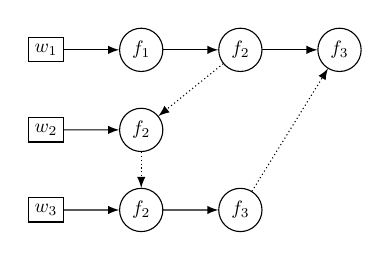
\begin{tikzpicture}[
roundnode/.style={circle, draw},
squarednode/.style={rectangle, draw},
every node/.append style={transform shape},
scale=0.7]
% Nodes
\node[squarednode] (w1) {\(w_1\)};
\node[squarednode] (w2) [below=of w1] {\(w_2\)};
\node[squarednode] (w3) [below=of w2] {\(w_3\)};
\node[roundnode] (f11) [right=of w1] {\(f_1\)};
\node[roundnode] (f12) [right=of f11] {\(f_2\)};
\node[roundnode] (f13) [right=of f12] {\(f_3\)};
\node[roundnode] (f22) [right=of w2] {\(f_2\)};
\node[roundnode] (f32) [right=of w3] {\(f_2\)};
\node[roundnode] (f33) [right=of f32] {\(f_3\)};
% Lines
\draw[arrows={-latex}] (w1) -- (f11);
\draw[arrows={-latex}] (f11) -- (f12);
\draw[arrows={-latex}] (f12) -- (f13);
\draw[arrows={-latex}] (w2) -- (f22);
\draw[arrows={-latex}] (w3) -- (f32);
\draw[arrows={-latex}] (f32) -- (f33);
\draw[densely dotted,arrows={-latex}] (f12) -- (f22);
\draw[densely dotted,arrows={-latex}] (f22) -- (f32);
\draw[densely dotted,arrows={-latex}] (f33) -- (f13);
\end{tikzpicture}
\column{0.3\textwidth}
\footnotesize{\textbf{Search Table} \(\mathtt{T}_s\)}
\(F_{K_1}(w_1) \rightarrow 4\)\\
\(F_{K_1}(w_2) \rightarrow 0\)\\
\(F_{K_1}(w_3) \rightarrow 5\)\\
\(\textsf{free} \rightarrow 6\)
\column{0.3\textwidth}
\footnotesize{\textbf{Deletion Table} \(\mathtt{T}_d\)}
\(F_{K_1}(f_1) \rightarrow 1\)\\
\(F_{K_1}(f_2) \rightarrow 5\)\\
\(F_{K_1}(f_3) \rightarrow 4\)
\end{columns}

\vspace{2ex}
\hrule
\includegraphics[trim=55mm 175mm 43mm 60mm, clip, width=0.9\textwidth]{../paper/pg_0005.pdf}
\end{center}
\end{frame}


\begin{frame}[fragile]
\frametitle{Example - Adding a file}

\begin{center}
\begin{columns}
\column{0.05\textwidth}
\column{0.4\textwidth}
\footnotesize{\textbf{Index}}\\
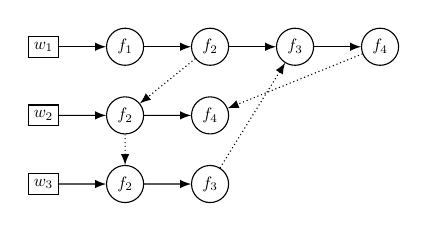
\begin{tikzpicture}[
roundnode/.style={circle, draw},
squarednode/.style={rectangle, draw},
every node/.append style={transform shape},
scale=0.6]
% Nodes
\node[squarednode] (w1) {\(w_1\)};
\node[squarednode] (w2) [below=of w1] {\(w_2\)};
\node[squarednode] (w3) [below=of w2] {\(w_3\)};
\node[roundnode] (f11) [right=of w1] {\(f_1\)};
\node[roundnode] (f12) [right=of f11] {\(f_2\)};
\node[roundnode] (f13) [right=of f12] {\(f_3\)};
\node[roundnode] (f14) [right=of f13] {\(f_4\)};
\node[roundnode] (f22) [right=of w2] {\(f_2\)};
\node[roundnode] (f24) [right=of f22] {\(f_4\)};
\node[roundnode] (f32) [right=of w3] {\(f_2\)};
\node[roundnode] (f33) [right=of f32] {\(f_3\)};
% Lines
\draw[arrows={-latex}] (w1) -- (f11);
\draw[arrows={-latex}] (f11) -- (f12);
\draw[arrows={-latex}] (f12) -- (f13);
\draw[arrows={-latex}] (f13) -- (f14);
\draw[arrows={-latex}] (w2) -- (f22);
\draw[arrows={-latex}] (f22) -- (f24);
\draw[arrows={-latex}] (w3) -- (f32);
\draw[arrows={-latex}] (f32) -- (f33);
\draw[densely dotted,arrows={-latex}] (f12) -- (f22);
\draw[densely dotted,arrows={-latex}] (f14) -- (f24);
\draw[densely dotted,arrows={-latex}] (f22) -- (f32);
\draw[densely dotted,arrows={-latex}] (f33) -- (f13);
\end{tikzpicture}
\column{0.3\textwidth}
\footnotesize{\textbf{Search Table} \(\mathtt{T}_s\)}
\(F_{K_1}(w_1) \rightarrow 4\)\\
\(F_{K_1}(w_2) \rightarrow 0\)\\
\(F_{K_1}(w_3) \rightarrow 5\)\\
\column{0.3\textwidth}
\footnotesize{\textbf{Deletion Table} \(\mathtt{T}_d\)}
\(F_{K_1}(f_1) \rightarrow 1\)\\
\(F_{K_1}(f_2) \rightarrow 5\)\\
\(F_{K_1}(f_3) \rightarrow 4\)\\
\(F_{K_1}(f_4) \rightarrow 3\)
\end{columns}

\vspace{2ex}
\hrule
\includegraphics[trim=55mm 175mm 73mm 60mm, clip, width=0.7\textwidth]{../paper/pg_0005_add.pdf}
\end{center}
\end{frame}


\begin{frame}[fragile]
\frametitle{Example - Deleting a file}

\begin{center}
\begin{columns}
\column{0.05\textwidth}
\column{0.4\textwidth}
\footnotesize{\textbf{Index}}\\
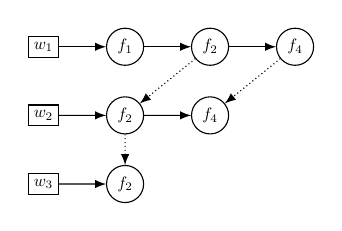
\begin{tikzpicture}[
roundnode/.style={circle, draw},
squarednode/.style={rectangle, draw},
every node/.append style={transform shape},
scale=0.6]
% Nodes
\node[squarednode] (w1) {\(w_1\)};
\node[squarednode] (w2) [below=of w1] {\(w_2\)};
\node[squarednode] (w3) [below=of w2] {\(w_3\)};
\node[roundnode] (f11) [right=of w1] {\(f_1\)};
\node[roundnode] (f12) [right=of f11] {\(f_2\)};
\node[roundnode] (f14) [right=of f12] {\(f_4\)};
\node[roundnode] (f22) [right=of w2] {\(f_2\)};
\node[roundnode] (f24) [right=of f22] {\(f_4\)};
\node[roundnode] (f32) [right=of w3] {\(f_2\)};
% Lines
\draw[arrows={-latex}] (w1) -- (f11);
\draw[arrows={-latex}] (f11) -- (f12);
\draw[arrows={-latex}] (f12) -- (f14);
\draw[arrows={-latex}] (w2) -- (f22);
\draw[arrows={-latex}] (f22) -- (f24);
\draw[arrows={-latex}] (w3) -- (f32);
\draw[densely dotted,arrows={-latex}] (f12) -- (f22);
\draw[densely dotted,arrows={-latex}] (f14) -- (f24);
\draw[densely dotted,arrows={-latex}] (f22) -- (f32);
\end{tikzpicture}
\column{0.3\textwidth}
\footnotesize{\textbf{Search Table} \(\mathtt{T}_s\)}
\(F_{K_1}(w_1) \rightarrow 4\)\\
\(F_{K_1}(w_2) \rightarrow 0\)\\
\(F_{K_1}(w_3) \rightarrow 5\)\\
\column{0.3\textwidth}
\footnotesize{\textbf{Deletion Table} \(\mathtt{T}_d\)}
\(F_{K_1}(f_1) \rightarrow 1\)\\
\(F_{K_1}(f_2) \rightarrow 5\)\\
\(F_{K_1}(f_4) \rightarrow 3\)
\end{columns}

\vspace{2ex}
\hrule
\includegraphics[trim=55mm 175mm 73mm 60mm, clip, width=0.7\textwidth]{../paper/pg_0005_del.pdf}
\end{center}
\end{frame}


\plain{Questions?}

\begin{frame}[allowframebreaks]
	\frametitle{References}
	\nocite{*}
	\bibliographystyle{abbrv}
	\bibliography{main}
\end{frame}

\end{document}
